\documentclass[tikz,border=6pt]{standalone}
\usepackage{amsmath}
\usetikzlibrary{arrows.meta,calc,patterns,positioning}
\begin{document}

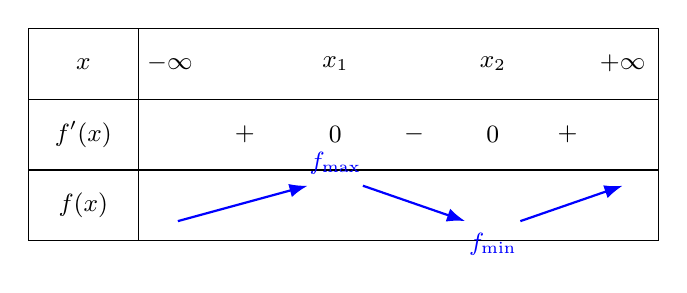
\begin{tikzpicture}[font=\small,>=Latex]
  \draw (0,0) rectangle (8,2.7);
  \draw (0,1.8) -- (8,1.8);
  \draw (0,0.9) -- (8,0.9);
  \draw (1.4,0) -- (1.4,2.7);
  \node at (0.7,2.25) {$x$};
  \node at (0.7,1.35) {$f'(x)$};
  \node at (0.7,0.45) {$f(x)$};
  \node at (1.8,2.25) {$-\infty$};
  \node at (3.9,2.25) {$x_1$};
  \node at (5.9,2.25) {$x_2$};
  \node at (7.55,2.25) {$+\infty$};
  \node at (2.75,1.35) {$+$};
  \node at (3.9,1.35) {$0$};
  \node at (4.9,1.35) {$-$};
  \node at (5.9,1.35) {$0$};
  \node at (6.85,1.35) {$+$};
  \draw[->,thick,blue] (1.9,0.25) -- (3.55,0.7);
  \draw[->,thick,blue] (4.25,0.7) -- (5.55,0.25);
  \draw[->,thick,blue] (6.25,0.25) -- (7.55,0.7);
  \node[above,blue] at (3.9,0.72) {$f_{\max}$};
  \node[below,blue] at (5.9,0.22) {$f_{\min}$};
\end{tikzpicture}

\end{document}
